\chapter{Estado da Arte}
\label{chap:EA}

O estado da arte refere-se ao conhecimento atual sobre um determinado tema em análise ou estudo. Este capítulo apresenta uma visão geral das origens do termo ESG, destacando os benefícios da adoção destas práticas, os desafios da sua implementação e monitorização, além de discutir o papel da tecnologia na gestão ESG.

Em seguida, é realizada uma análise dos trabalhos relacionados com a temática do projeto, acompanhada de uma compilação das tecnologias já existentes para a avaliação e gestão de métricas ESG.

%-------------------------------------------------------------------------------

\section{ESG - história do conceito e aplicação} 
\label{sec:OESG} 

O conceito de \gls{ESG} surgiu na década de \textbf{1990}, quando a \gls{ONU} passou a adotar uma postura mais aberta em relação ao setor corporativo. Durante esse período, o então Secretário-Geral da ONU, Kofi Annan, lançou as bases da iniciativa que levaria à criação do conceito de ESG. No contexto da missão das Nações Unidas de promover a paz e o desenvolvimento, aliada aos objetivos do setor empresarial de gerar riqueza e prosperidade, a organização começou a estabelecer parcerias estratégicas, reconhecendo o papel fundamental das empresas no avanço desses objetivos (\cite{Pollman2024}).

Em \textbf{1999}, durante o Fórum Econômico Mundial de Davos, Kofi Annan apresentou a proposta \textit{Global Compact} (\cite{Pollman2024}), que se tornou operacional em \textbf{2000}, de interesse mútuo da ONU e do setor corporativo. De acordo com a \gls{ONU}, trata-se de "um apelo às empresas para alinharem as suas estratégias e operações com princípios universais de direitos humanos, trabalho, meio ambiente e combate à corrupção, e tomem medidas que promovam objetivos sociais" (\cite{ONUGC2025}). Esta iniciativa tem por base dez princípios fundamentados nos direitos humanos, trabalho, meio ambiente e combate à corrupção \footnote{Os princípios que constituem a iniciativa \textit{Global Compact} estão disponíveis no site oficial \textit{UN Global Compact}: \url{https://unglobalcompact.org/what-is-gc/mission/principles} (acesso a 31/03/2025).}.

\subsection{Who Cares Wins}
\label{subsec: WCW}

Em \textbf{2004}, Kofi Annan convidou algumas das principais instituições financeiras do mundo para se unirem à \gls{ONU} numa nova iniciativa, como extensão do \textit{Global Compact}: o projeto \textit{Who Cares Wins}.

Esta iniciativa reuniu, pela primeira vez, investidores institucionais, gestores de ativos, analistas de pesquisa buy-side\footnote{Buy-side refere-se a instituições que compram ativos para investimento próprio, como fundos de investimento e seguradoras.} e sell-side\footnote{Sell-side refere-se a instituições que vendem ativos e oferecem recomendações de investimento, como corretoras e bancos de investimento.}, consultores globais, órgãos governamentais e reguladores, com o objetivo de examinar o papel dos fatores \gls{ESG} na gestão de ativos e na pesquisa financeira (\cite{Pollman2024}).

Como resultado, chegou-se a um consenso sobre o impacto dos fatores ESG no contexto de investimentos de longo prazo, e foi elaborado um relatório\footnote{Uma versão em PDF do relatório de 2004 está disponível em \url{https://www.ifc.org/content/dam/ifc/doc/mgrt/whocareswins-2005conferencereport.pdf} (acesso a 31/03/2025).}, no qual o termo "ESG" foi introduzido oficialmente. O documento também apresentou recomendações para diferentes atores do mercado sobre como integrar questões ambientais, sociais e de governança corporativa na gestão de ativos, nos serviços de corretagem de valores mobiliários\footnote{Corretagem de valores mobiliários refere-se à intermediação na compra e venda de ativos financeiros, normalmente realizada por corretoras.} e nas funções de pesquisa associadas (\cite{onValues2005}).

\begin{figure}[h]
    \centering
    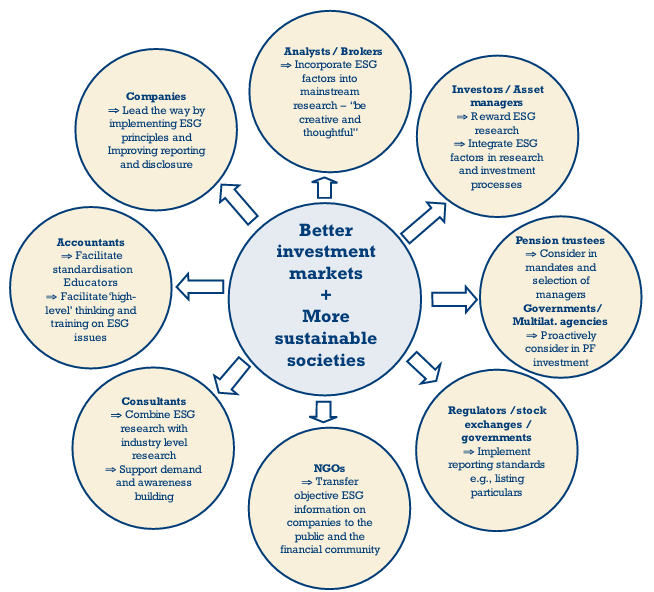
\includegraphics[width=5in]{frontmatter/assets/agentes-chave-esg-wcw.png}
    \caption{Principais intervenientes envolvidos na integração de temáticas ESG segundo o relatório \textit{Who Cares Wins} (\cite{onValues2005})}
    \label{fig:wcwactors}
\end{figure}

Segundo \cite{Pollman2024}, "embora o termo ESG tenha sido mencionado em menos de 1\% das conferências de resultados financeiros nos anos seguintes ao relatório \textit{Who Cares Wins}, em 2021 a sua presença cresceu significativamente, sendo citado em quase um quinto dessas conferências. Além disso, um estudo revelou que 72\% dos investidores institucionais passaram a incorporar fatores ESG nas suas estratégias".

\subsection{PRI: Princípios de Investimento Responsável}
\label{subsec: PRI}

Com a crescente conscientização dos problemas ESG, surgiram outras iniciativas, como os \gls{PRI}. O PRI foi iniciado em \textbf{2005} por Kofi Annan, que convidou um grupo internacional de investidores institucionais a desenvolver iniciativas que refletissem a crescente importância das questões ESG nas práticas de investimento (\cite{Kim2022}).

Os PRI mantêm uma forte ligação à \gls{ONU} através dos seus dois parceiros fundadores — o UN Global Compact e a UNEP Finance Initiative (UNEP FI). A iniciativa assenta em seis princípios \footnote{Os seis princípios para investimento responsável podem ser consultados no site oficial: \url{https://www.unpri.org/about-us/what-are-the-principles-for-responsible-investment} (acesso em 31/03/2025).} concebidos para reforçar a relação entre o investimento responsável e o desenvolvimento sustentável, alinhando o trabalho do PRI com os Objetivos de Desenvolvimento Sustentável (ODS)\footnote{As Nações Unidas disponibilizam um website com informações detalhadas sobre os ODS: \url{https://ods.pt/ods/} (acesso em 31/03/2025).} e incentivando os seus signatários a adotar a mesma abordagem (\cite{PRIBlueprint2017}).

No seu website\footnote{O site oficial do PRI disponibiliza informações detalhadas sobre as várias medidas, práticas e desafios ESG. As \textbf{questões ambientais} podem ser consultadas em \url{https://www.unpri.org/sustainability-issues/environmental-social-and-governance-issues/environmental-issues}, as \textbf{questões sociais} em \url{https://www.unpri.org/sustainability-issues/environmental-social-and-governance-issues/social-issues} e as \textbf{questões de governança} em \url{https://www.unpri.org/sustainability-issues/environmental-social-and-governance-issues/governance-issues} (acesso em 31/03/2025).}, os \gls{PRI} enumeram uma vasta gama de desafios, temáticas e externalidades ESG que as empresas devem considerar cada vez mais. Estes desafios abrangem três grandes dimensões:

\begin{itemize}
\item \textbf{Ambiente} – conservação da natureza, transição para uma economia circular, gestão sustentável da água, impactos do fraturamento hidráulico e emissões de metano.
\item \textbf{Sociedade} – promoção da diversidade, equidade e inclusão, bem como condições de trabalho dignas.
\item \textbf{Governança} – justiça tributária, engajamento político responsável, segurança cibernética, remuneração executiva, propósito corporativo, combate à corrupção, proteção de denunciantes e nomeações de diretores.
\end{itemize}

%-------------------------------------------------------------------------------

\section{Trabalhos relacionados} 
\label{sec:TR} 

Esta secção tem como objetivo apresentar o estado da arte sobre ESG, abordando tanto os desafios e impactos desses fatores nas empresas quanto as soluções já desenvolvidas para sua análise e reporte. Para isso, será feita uma revisão de artigos científicos e tecnologias aplicadas ao mercado.  

Primeiramente, serão exploradas as práticas ESG e os seus efeitos no valor, rentabilidade e riscos das empresas, com base em estudos recentes sobre a relação entre desempenho financeiro e fatores ESG. Em seguida, serão analisadas as principais metodologias e abordagens utilizadas para reporte e análise ESG, destacando a diversidade de métricas e frameworks existentes e os desafios relacionados à sua padronização.  

Posteriormente, serão discutidas as tendências atuais, com ênfase no impacto das novas tecnologias, como inteligência artificial e análise de dados em tempo real, na otimização da gestão ESG. A secção também apresentará um levantamento das principais tecnologias disponíveis no mercado, incluindo frameworks de relato ESG e softwares especializados.  

Por fim, será introduzido o contexto tecnológico da solução proposta, destacando as ferramentas e bibliotecas utilizadas no seu desenvolvimento e justificando a escolha dessas tecnologias com base nas necessidades do projeto.

%-------------------------------------------------------------------------------

\subsection{Práticas e Riscos ESG: Impacto no Valor e Rentabilidade das Empresas}
\label{subsec:PESGE}

O movimento por detrás da sigla ESG é bastante complexo, incorporando elementos de responsabilidade social, ambiental e governança corporativa para avaliar empresas. Os fatores de \gls{ESG} são importantes para medir a sustentabilidade dos agentes econômicos e expandem o escopo do desempenho corporativo. Fatores externos, como o mercado e a indústria, e fatores internos, como a estrutura de propriedade e o conselho de administração, influenciam as práticas ESG na criação de valor (\cite{Wang2023}).

Segundo uma análise conduzida por \cite{Whelan2021}, em colaboração com a \textit{Rockefeller Asset Management} e o \textit{NYU Stern Center for Sustainable Business}, examinou-se mais de 1000 estudos publicados entre 2015 e 2020 sobre a relação entre fatores ESG e desempenho financeiro. Os resultados indicaram que 58\% dos estudos identificaram uma relação positiva, 8\% uma relação negativa, 13\% nenhuma relação e 21\% apresentaram resultados mistos. Embora a maioria dos estudos sugira um impacto positivo dos fatores ESG no desempenho financeiro, os autores concluem que os resultados refletem um debate contínuo sobre o tema.

Os estudos que identificaram uma \textbf{relação positiva} entre práticas ESG e desempenho financeiro apontam uma forte correlação entre a qualidade dos relatórios ESG e o valor da empresa. Isso sugere que a transparência, a confiança e a responsabilização dos \textit{stakeholders} exercem uma influência positiva na valorização da empresa (\cite{Aydomu2022}).

Por outro lado, os estudos que encontraram \textbf{efeitos negativos} destacam diferentes fatores. Entre eles, está o impacto adverso no desempenho financeiro devido à realocação de recursos dos acionistas (\textit{shareholders}) para outras partes interessadas (\textit{stakeholders}). Além disso, há evidências de que, em mercados emergentes, a relação entre pontuações ESG e retorno financeiro tende a ser negativa, possivelmente devido a desafios estruturais e regulatórios nesses mercados (\cite{Aydomu2022}).

Os estudos que relataram \textbf{efeitos mistos} destacam que o impacto do relato sobre temáticas ambientais tende a ser negativo para o desempenho financeiro da empresa. Em contrapartida, a participação ativa dos \textit{stakeholders} na gestão demonstra uma correlação positiva com a dimensão social, enquanto a governança também se mostra favorável ao desempenho financeiro. De forma geral, observa-se uma predisposição positiva na relação entre os níveis de ESG e o valor da empresa, ainda que esse impacto não se reflita diretamente na rentabilidade (\cite{Aydomu2022}).

Segundo \cite{Aydomu2022}, "a pontuação combinada de métricas ESG tem uma relação positiva e altamente significativa com o valor da empresa", porém a dimensão ambiental não acompanha esse mesmo padrão. O estudo sugere que, ao contrário dos componentes sociais e de governança, as iniciativas ambientais levam mais tempo—por vezes anos—para gerar resultados concretos para a empresa. Além disso, os elevados custos de investimento associados às práticas ambientais podem representar um obstáculo, tornando esta dimensão menos atrativa em termos de impacto financeiro imediato. Estatísticas descritivas do estudo indicam que a média da pontuação ambiental tende a ser inferior às pontuações de governança e social, o que reforça a ideia de que essa métrica evolui de forma mais lenta e exige investimentos mais significativos.

De acordo com \cite{Cohen2023}, a pontuação ESG indica que empresas de maior dimensão tendem a ser menos poluentes. No entanto, apresentam menor preocupação com as implicações sociais de suas operações e enfrentam desafios crescentes em governança. O estudo destaca que, à medida que expandem as suas operações globalmente, os conglomerados passam a priorizar questões ambientais. Contudo, a governança torna-se mais complexa, devido às dificuldades no controlo corporativo de empresas internacionais de grande porte, evidenciando os desafios inerentes à sua gestão.

% %-------------------------------------------------------------------------------

\subsection{Métodos e abordagens para reporte e análise ESG}
\label{subsec: MARAESG}

Com o crescimento das preocupações em torno das métricas \gls{ESG}, surgiram diversas classificações amplamente utilizadas, desenvolvidas por provedores de dados \footnote{Entidades que atuam como intermediários na coleta, armazenamento e distribuição de dados, como provedores de serviços de internet, empresas de telecomunicações ou plataformas online.} ESG para auxiliar investidores na comparação e avaliação do desempenho das empresas nesses critérios. Inicialmente, os dados ESG eram obtidos a partir de fontes públicas, como relatórios financeiros e sites corporativos. No entanto, com o aumento das exigências de transparência, um número crescente de empresas passou a publicar relatórios anuais de \gls{CRS}, o que contribui para a ampliação da disponibilidade de dados ESG. Apesar desse avanço, a qualidade e confiabilidade das informações continuam sendo motivo de preocupação. Os indicadores divulgados frequentemente apresentam inconsistências entre diferentes empresas, dificultando comparações diretas e resultando em divergências entre as agências de classificação ESG (\cite{Rau2024}).

A forma como as agências de classificação ESG avaliam as empresas depende das informações divulgadas e dos critérios adotados para a medição. No entanto, há divergências significativas em relação ao escopo, à ponderação dos fatores e aos métodos de avaliação utilizados por cada agência. O escopo e o peso determinam quais aspectos uma classificação ESG busca medir, enquanto a medição define a forma como esses aspectos são avaliados. A principal fonte de discrepância entre as classificações ESG está na divergência dos critérios de medição, refletindo diferenças nas perspectivas das agências sobre quais categorias devem ter maior relevância na avaliação do desempenho ESG de uma empresa (\cite{Berg2022}).

Em resposta à crescente demanda por informações não financeiras mais confiáveis, mensuráveis e transparentes, diversas \textit{frameworks} de sustentabilidade —como os \textit{UN SDGs, GRI, IIRC} e \textit{SASB}— foram desenvolvidas e implementadas. O objetivo comum destas estruturas é padronizar a divulgação de informações ambientais, sociais e de governança (ESG), permitindo maior comparabilidade entre as empresas. Embora a maioria destas \textit{frameworks} seja de adoção voluntária e tenha um foco seletivo em alguns aspetos, elas buscam oferecer padrões de alta qualidade que diferenciem empresas genuinamente comprometidas com a melhoria de seu desempenho sustentável daquelas que praticam \textit{greenwashing} (\cite{Cruz2023}).

O \textit{greenwashing}\footnote{\textit{Top-Performing Singapore Firm Accused of Greenwashing in India Coal Sale}" \url{https://www.bloomberg.com/news/articles/2022-11-09/top-performing-singapore-stock-with-temasek-backing-is-accused-of-greenwashing}} surge como um efeito colateral das preocupações das empresas com a sua imagem, ocorrendo quando estas tentam projetar uma reputação pró-sustentabilidade e afirmam adotar práticas ESG, mas falham em cumprir efetivamente as suas responsabilidades. Esta prática pode manifestar-se de diversas formas, incluindo narrativas ou divulgações seletivas e enganosas, alegações ambientais sem fundamento, certificações e rótulos duvidosos, entre outras estratégias que induzem os consumidores e investidores a percepções distorcidas sobre o real impacto da empresa (\cite{Rau2024}).

Segundo \cite{Schiemann2022}, uma maior divulgação ESG por parte das empresas está associada a níveis mais elevados de controvérsias ESG. Empresas envolvidas em controvérsias ESG enfrentam maior incerteza na precisão das previsões analíticas, afetando a confiança de investidores. No entanto, a divulgação ESG desempenha um papel moderador nesta relação: uma comunicação transparente e detalhada pode mitigar a incerteza gerada pelas controvérsias, reduzindo os impactos negativos na percepção do mercado. Estes resultados possuem implicações práticas tanto para investidores, que buscam informações mais confiáveis, quanto para as empresas, que podem utilizar a divulgação ESG como estratégia para fortalecer a sua credibilidade.

%-------------------------------------------------------------------------------

\subsection{Tendências atuais em ESG e tecnologia}
\label{subsec: TAESG}

Um estudo realizado por \cite{Krueger2024} observou os efeitos de divulgação ESG na liquidez de ações das empresas, sendo a sua amostra constituída por 17 680 empresas únicas em 65 países no período entre 2002 e 2020. O artigo conclui que mandatos de divulgação ESG obrigatórios têm um efeito positivo significativo na liquidez de ações, particularmente quando implementados por instituições governamentais numa base de conformidade total e aplicados por instituições informais.

O crescimento da relevância deste tópico ao longo das últimas duas décadas ocorreu em paralelo com uma revolução tecnológica contínua. A digitalização das empresas tem proporcionado diversos benefícios às práticas ESG no contexto corporativo, resultando em melhorias significativas nas suas pontuações ESG. Entre as vantagens, destaca-se a redução dos custos de agência e o aumento das pontuações de governança e sociais. No entanto, não se observa uma correlação entre a digitalização das empresas e a melhoria das suas pontuações ambientais (\cite{Fang2023}).

A nova revolução tecnológica, conhecida como Indústria 5.0, impulsionou a digitalização das empresas e forneceu-lhes ferramentas para uma divulgação ESG mais eficaz. Diferenciando-se da Indústria 4.0, cujo foco era essencialmente económico e técnico, a Indústria 5.0 enfatiza a gestão humana e a sustentabilidade. O seu cerne inclui a \textbf{centralidade no ser humano} (promoção de um ambiente de trabalho seguro e saudável), a \textbf{sustentabilidade} (preservação de recursos e crescimento equilibrado) e a \textbf{resiliência} (capacidade de recuperação frente a interrupções). Assim, os princípios da Indústria 5.0 estão intrinsecamente alinhados às temáticas ESG. A Indústria 5.0 aprimora a autenticidade e a abrangência da divulgação ESG ao transformar relatórios retrospectivos em prospectivos e em tempo real. Ela possibilita personalizações nos relatórios ESG, expande o escopo da divulgação para cadeias de suprimentos multicamadas, reduz os custos ESG e melhora a eficácia geral dessas divulgações.  (\cite{Asif2023}).

No âmbito técnico, a Indústria 5.0 engloba diversas tecnologias que otimizam o fluxo e o compartilhamento de informações, tais como sensores, RFID\footnote{RFID (\textit{radio frequency identification}) é uma tecnologia sem fio que usa ondas de rádio para identificar de forma exclusiva objetos, animais ou pessoas.} e IoT\footnote{Internet das Coisas (IoT) refere-se a uma rede de dispositivos físicos, veículos, aparelhos e outros objetos incorporados com sensores, software e recursos de conectividade, permitindo-lhes coletar e trocar dados pela Internet.}; transações descentralizadas via \textit{blockchain}\footnote{\textit{Blockchain} é uma tecnologia de registro digital descentralizado, onde informações são armazenadas em blocos interligados, formando uma cadeia. Cada bloco contém dados e uma referência ao bloco anterior, tornando difícil alterar as informações sem afetar toda a cadeia, garantindo segurança e transparência nas transações.}; processamento de grandes volumes de dados utilizando \textit{big data} e computação em nuvem; tomada de decisão inteligente com apoio de \textit{machine learning}, IA e simulações; além da automação de processos com robôs e drones (\cite{Asif2023}).

Atualmente, a inteligência artificial (IA) é uma área tecnológica em rápido crescimento que envolve métodos numéricos para resolver diversos problemas de previsão, otimização e classificação/agrupamento. De acordo com \cite{Burnaev2023}, foi realizado um estudo sobre o uso prático da IA para enfrentar desafios ESG. Algoritmos de IA podem acelerar o processamento de dados e aprimorar a compreensão das informações extraídas, contribuindo significativamente para questões ambientais, sociais e de governança. Alguns dos casos práticos encontrados no estudo incluem: IA ajuda a atingir até 93\% das metas dos Objetivos de Desenvolvimento Sustentável (ODS) no domínio ambiental, como ações climáticas, monitorização de desastres e redução da poluição; o uso de IA em cidades inteligentes, com destaque para redes elétricas inteligentes, manutenção preditiva e ambientes centrados no ser humano; a IA é aplicada para detetar evasão fiscal e práticas de \textit{greenwashing}; e, para investidores, a IA permite avaliar o desempenho das empresas com base nos comunicados públicos, relatórios e artigos por meio de \gls{PNL}\footnote{Processamento de Linguagem Natural (PNL) é um campo da inteligência artificial que se concentra na interação entre computadores e a linguagem humana. Este envolve a capacidade dos sistemas computacionais de entender, interpretar e gerar texto ou fala de forma que seja útil para os utilizadores, aplicando técnicas como a análise de sentimentos, a tradução automática e o reconhecimento de voz.}. O PNL também automatiza rotinas de tarefas, como verificar a consistência de documentos e gerar relatórios.

%------------------------------------------------------------------------------- 

\section{Tecnologias existentes} 
\label{sec:TechExist}

A presente secção do relatório tem como objetivo documentar as tecnologias existentes, justificando as decisões e escolhas feitas na implementação da solução. Inicia-se com uma análise das \textit{frameworks} de relato ESG mencionadas na descrição do projeto, e inclui uma comparação entre estas. De seguida, realiza-se uma pesquisa sobre os principais \textit{softwares} ESG disponíveis no mercado. Por fim, é feita uma breve menção ao \textit{React} e às bibliotecas utilizadas na implementação do projeto.

%-------------------------------------------------------------------------------
\subsection{Frameworks de Relato ESG}
\label{subsec: FRESG}

Diversas \textit{frameworks} de sustentabilidade/ESG foram criadas para padronizar a divulgação de informações não financeiras, tornando-as mais fiáveis e acessíveis aos investidores. Apesar de serem maioritariamente voluntárias, estas estruturas facilitam a avaliação do impacto da sustentabilidade nas empresas e ajudam a distinguir compromissos reais de \textit{greenwashing} (\cite{Cruz2023}).

\subsubsection{GRI (Global Reporting Initiative)}
\label{subsubsec: GRI}

A \gls{GRI} é uma \textit{framework} cujo público-alvo são os grupos de partes interessadas (\textit{stakeholders}) (\cite{GRISASB2021}), e foi a primeira das iniciativas a surgir, tornando-se a principal referência para a elaboração de relatórios a nível mundial (\cite{Luque-Vlchez2023}).

A \textit{framework} GRI consiste num sistema modular de normas que distingue entre requisitos ("\textit{shall}"), recomendações ("\textit{should}") e orientações (\cite{Adams2022}). A \gls{GRI} organiza-se em três tipos de normas\footnote{O site oficial da \gls{GRI} detalha as normas da \textit{framework}: \url{https://www.globalreporting.org/media/s4cp0oth/gri-gristandards-visuals-fig1_family-2021-print-v19-01.png} e \url{https://www.globalreporting.org/how-to-use-the-gri-standards/gri-standards-english-language/} (acesso em 04/04/2025)}: normas universais, normas setoriais e normas para tópicos específicos (\cite{GRI2025}). As organizações começam com as normas universais, utilizam depois a(s) norma(s) sectorial(ais) aplicável(eis) para determinar os tópicos materiais e relatam-nos utilizando as normas temáticas relevantes (\cite{GRISector2025}).

A estrutura modular da \textit{framework} proporciona maior flexibilidade e uma abordagem mais detalhada na divulgação ESG das empresas. O seu objetivo principal é promover transparência e responsabilidade sobre os impactos empresariais, além de facilitar um diálogo mais informado sobre sustentabilidade corporativa. A GRI busca, assim, estabelecer um idioma comum para relatórios de impacto, auxiliando na construção de um futuro sustentável (\cite{Adams2022}).

A GRI é uma \textit{framework} em constante expansão. O seu programa \textit{GRI Sector Program} tem como objetivo desenvolver normas específicas para 40 setores\footnote{A GRI disponibilizou um documento sobre o \textit{GRI Sector Program}, onde cataloga e agrega setores de acordo com a sua prioridade: \url{https://www.globalreporting.org/media/mqznr5mz/gri-sector-program-list-of-prioritized-sectors.pdf} (acesso em 04/04/2025)}, começando pelos que mais contribuem para as necessidades básicas e, posteriormente, expandindo-se para setores adjacentes (\cite{GRISector2025}).

%-------------------------------------------------------------------------------

\subsubsection{SASB (Sustainability Accounting Standards Board)}
\label{subsubsec: SASB}

A \gls{SASB} é uma \textit{framework} cujo público-alvo são os investidores (\cite{GRISASB2021}). Embora seja de caráter voluntário, foi adotada globalmente e é composta por conjuntos de normas que padronizam 77 indústrias\footnote{O documento indicado pelo URL refere-se às normas SASB de divulgação ESG para a indústria de \textit{software} e serviços IT, onde se enquadra a Devscope. \url{https://d3flraxduht3gu.cloudfront.net/latest_standards/software-and-it-services-standard_en-gb.pdf} (acesso em 04/04/2025)} (\cite{SASB2025}). O foco da SASB é estabelecer e fornecer normas para a divulgação de informações sobre questões de sustentabilidade, facilitando a comunicação de dados não financeiros relevantes entre as empresas e os investidores (\cite{Goswami2023}). A \textit{framework} considera os impactos no curto, médio e longo prazo sobre o valor das empresas.

Segundo \cite{Cruz2023}, um dos componentes mais importantes desta \textit{framework} é o \textbf{“Mapa de Materialidade”}\footnote{\url{https://sasb.ifrs.org/standards/materiality-map/}}, que oferece informações claras e acessíveis sobre quais as questões de sustentabilidade que são materiais para setores específicos. Isto permite que os investidores tenham acesso a informações diretamente, sem a necessidade de realizar uma análise extensa para avaliar a materialidade financeira de uma empresa nas questões ESG.

%-------------------------------------------------------------------------------

\subsubsection{GRI e SASB: Diferenças-Chave e Complementaridade}
\label{subsubsec: GRI_E_SASB}

Como mencionado nas subsecções anteriores, tanto a \gls{GRI} quanto a \gls{SASB} são \textit{frameworks} cujo objetivo é compilar informações de forma normalizada, visando melhorar a divulgação e a pontuação ESG das empresas, assim como avaliar seu valor, rentabilidade e performance consoante questões ESG.

Em \textbf{2021}, ambas as organizações por detrás das \textit{frameworks} uniram-se para estudar o uso das suas normas no mercado, assim como averiguar as diferenças entre si e a sua complementaridade (\cite{GRISASB2021}). De acordo com \cite{GRISASB2021}, \cite{Pizzi2023} e \cite{Antolin-Lopez2023}, as diferenças destacadas foram:

\begin{table}
    \centering
    \begin{tabular}{|p{3cm}|p{5cm}|p{5cm}|}
        \hline
        \textbf{Critério} & \textbf{GRI} & \textbf{SASB} \\
        \hline
        \textbf{Aplicação da Materialidade} & Prioriza a divulgação de tópicos com impactos económicos, ambientais, sociais e de direitos humanos significativos. & Foca em informações financeiramente relevantes que possam influenciar decisões de investimento e crédito. \\
        \hline
        \textbf{Tipo e Âmbito da Divulgação} & Aborda os impactos económicos, ambientais e sociais das atividades da empresa no desenvolvimento sustentável global. & Considera como os fatores sociais e ambientais afetam o valor da empresa, mas não o impacto da empresa no mundo. \\
        \hline
        \textbf{Público-Alvo} & \textit{Stakeholders} (partes interessadas em geral). & Investidores. \\
        \hline
        \textbf{Processo de Definição das Normas} & Desenvolvidas por grupos de peritos representando diversos interesses globais, com transparência total e consulta pública. & Baseadas em pesquisa com participação de empresas, investidores e especialistas, com avaliação baseada em evidências e processo transparente. \\
        \hline
    \end{tabular}
    \caption{Comparação entre GRI e SASB}
    \label{tab:gri_sasb}
\end{table}

Referenciando novamente o estudo conduzido por \cite{GRISASB2021}, diversos inquiridos consideram que ambos os conjuntos de normas são complementares, pois possibilitam uma divulgação mais abrangente das questões ESG a partir de diferentes perspetivas, abordagens à materialidade e grupos de interessados. Desta forma, as empresas conseguem atender tanto às necessidades dos investidores quanto das demais partes interessadas (\textit{stakeholders}).

%-------------------------------------------------------------------------------

\subsection{Softwares ESG e Soluções no Mercado}
\label{subsec: SESGSM}

A presente subsecção explora soluções no mercado que tratam de métricas e relatos ESG.

\subsubsection{Workiva}

A Workiva oferece uma plataforma cloud para relatórios financeiros, ESG, auditoria e conformidade, permitindo a recolha, gestão e comunicação de dados de forma integrada e segura. A solução centraliza workflows, automatiza processos e assegura a rastreabilidade e conformidade com diversas \textit{frameworks} e normas (\cite{Workiva2025}).

% \begin{figure}[h]
%     \centering
%     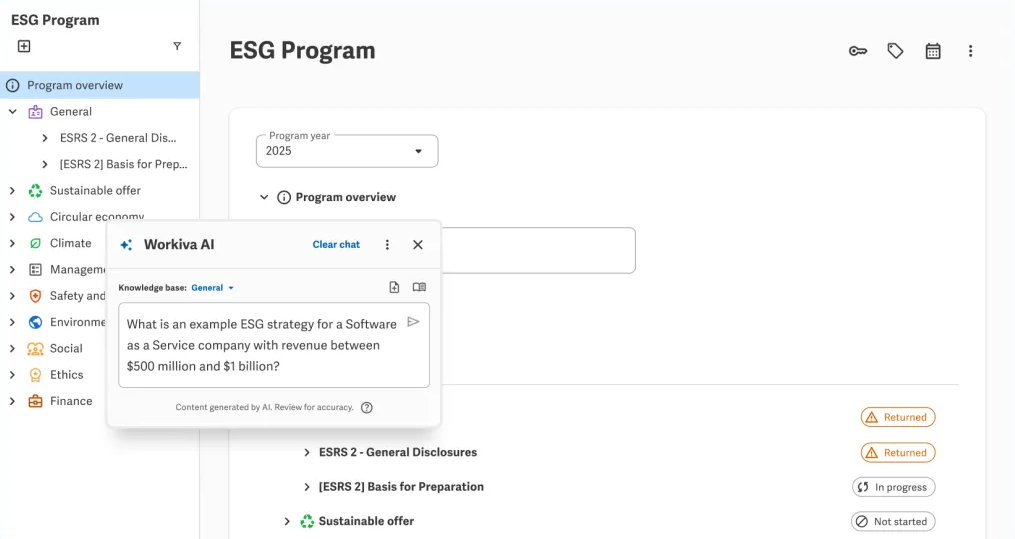
\includegraphics[width=5in]{frontmatter/assets/workiva.png}
%     \caption{Plataforma Workiva}
%     \label{fig:workiva}
% \end{figure}

\subsubsection{SAP Sustainability Control Tower}

O \textit{SAP Sustainability Control Tower} é uma solução SaaS\footnote{O SaaS, ou \textit{Software as a Service}, é um modelo de fornecimento de software baseado na nuvem (\textit{cloud}) em que os utilizadores acedem às aplicações através da Internet, em vez de as instalarem  localmente.} que permite às empresas registar, reportar e agir sobre métricas ESG com dados fiáveis e prontos para auditoria. Automatiza a integração de dados de múltiplas fontes, fornece cálculos avançados de emissões e incorpora \textit{insights} de sustentabilidade nos processos empresariais para uma gestão estratégica e transparente (\cite{SAP2025}).

\subsubsection{IBM Environmental Intelligence Suite}

O \textit{IBM Environmental Intelligence Suite} oferece APIs avançadas para integrar, analisar e visualizar dados ambientais, climáticos e de emissões de GEE\footnote{Emissões de gases com efeito de estufa (GEE).}. Ao usar \textit{machine learning} e \textit{AI-driven insights}, a plataforma permite extrair informações estratégicas, prever impactos e garantir conformidade com normas de sustentabilidade, adaptando-se às necessidades específicas de cada empresa (\cite{IBM2025}).

%-------------------------------------------------------------------------------
\subsection{Bibliotecas e Ferramentas de Desenvolvimento}
\label{subsec: BFD}

Esta subsecção aborda brevemente as ferramentas principais que serão usadas na solução desenvolvida.

\subsubsection{React.js}

O \textbf{React.js} é uma das bibliotecas\footnote{No contexto do \textit{React.js}, uma biblioteca é um conjunto de funcionalidades que pode utilizar para obter resultados que normalmente exigiriam mais código e trabalho da parte do utilizador.} \textit{JavaScript} de \textit{front-end} mais populares (\cite{Schwarzmuller2022}). O seu uso é focado na criação de interfaces de utilizador a partir de excertos de código individuais chamados \textbf{componentes} e das suas combinações em telas inteiras, páginas e aplicativos (\cite{React2025}).

\subsubsection{ApexCharts.js}

A \textbf{ApexCharts.js} é uma biblioteca de gráficos interativos \textit{open-source} em \textit{JavaScript}. Responsiva e de alto desempenho, permite criar visualizações dinâmicas com suporte a \textit{zoom}, \textit{scroll}, anotações e animações suaves. Oferece personalização avançada, incluindo gradientes, sombras e paletas de cores configuráveis, tornando-se uma solução eficiente para a visualização de dados na web (\cite{Apexcharts2025}).


 \vspace{20mm} 




